\documentclass[aps,pre,12pt,preprint,%
	onecolumn,showpacs,showkeys,nofootinbib]{revtex4-2}
%Chinese
	\usepackage[UTF8,fontset=fandol]{ctex}
%	\usepackage[datesep=/]{datetime2} % Use default
	\DeclareTextFontCommand{\textbf}{\sffamily}
%Presenting
	\usepackage[table]{xcolor}
	\usepackage{graphicx}
	\usepackage[font=small,format=plain,%
		labelfont=bf,textfont=it,%
		singlelinecheck=false]{caption}
	\usepackage[above]{placeins}
%	\usepackage{float} % Cause trouble for table footnotes
	\usepackage{wrapfig}
	\usepackage{tabularx,array,booktabs,multirow,bigstrut}
	\newcolumntype{C}[1]{>{\hsize=#1\hsize%
		\centering\arraybackslash}X}
	\newcommand{\minitab}[2][l]{%
		\begin{tabular}{#1}#2\end{tabular}}
	\usepackage{setspace,dcolumn}
	\usepackage{subfig}
	\usepackage{psfrag,epsfig}
%MathSetting
	\let\latexointop\ointop
	\usepackage{amsmath,bm,amssymb,esint,extarrows}
	\usepackage{upgreek,textcomp,mathrsfs}
	\usepackage[only,sslash]{stmaryrd}
	\usepackage{nicefrac,eqnarray}
%	\usepackage{amsthm} % Enable when necessary
%	\usepackage[mathscr]{eucal} % Enable when necessary
	\usepackage{mathtools,physics,siunitx}
	\usepackage{stackengine,varwidth}
	\usepackage{tikz}
	\usepackage{resizegather,empheq}
	\usetagform{default}
	\usepackage{calligra,fourier-orns}
	% Keep \oint unchanged by esint
	\let\ointop\undefined
	\let\ointop\latexointop
	% Define a scriptr 
	\DeclareMathAlphabet{\mathcalligra}{T1}{calligra}{m}{n}
	\DeclareFontShape{T1}{calligra}{m}{n}{<->s*[2.2]callig15}{}
	\newcommand{\scriptr}{\mathcalligra{r}\,}
	\newcommand{\rvector}{\pmb{\mathcalligra{r}}\,}
	% Useful shorthand
	\DeclarePairedDelimiter\ave{\langle}{\rangle}
	\newcommand\inlineeqno{\stepcounter{equation}\ (\theequation)}
	\newcommand{\sinc}{\operatorname{sinc}}
	\newcommand{\mbb}[1]{\mathbb{#1}}
	\newcommand{\mrm}[1]{\mathrm{#1}}
	\newcommand{\mcal}[1]{\mathcal{#1}}
	% Scaling and positioning
	\newcommand\scalemath[2]{\scalebox{#1}{\mbox{\ensuremath{\displaystyle #2}}}}
	\newcommand\raisemath[2]{\raisebox{#1\depth}{${#2}$}}
	\empheqset{box=\nicebox}
	% Presenting
	\newcommand*\nicebox[1]{\fbox{\hspace{1em}\addstackgap[5pt]{#1}\hspace{1em}}}

	\allowdisplaybreaks[2]
%ParagraphSetting
	\setlength{\parskip}{.3\baselineskip}
	\usepackage[defaultlines=2,all]{nowidow}
	\postdisplaypenalty=50
%PageSetting
	\usepackage{titlesec}
	\titleformat*{\section}{\large\bfseries}
	\usepackage[colorlinks=true,linkcolor=blue]{hyperref}
	\newcommand{\texstringonly}[1]{%
		\texorpdfstring{#1}{}}
	\usepackage[vmargin={3.5cm,4cm},hmargin=3cm,%
		footnotesep=\baselineskip]{geometry}
%	\usepackage[bottom]{footmisc} % Cause trouble for table footnotes
	\usepackage{changepage}
	% Autoref names
	\renewcommand{\tableautorefname}{\tablename}
	\renewcommand{\figureautorefname}{\figurename}
	% List settings
	\usepackage{enumitem}
	\setlist{itemsep=0pt,topsep=0pt,labelindent=\parindent,leftmargin=0pt,itemindent=*}
	% Some redefined lengths
	\setlength{\headsep}{1.6\baselineskip}
%	\setlength{\footnotesep}{3\parskip} % Use when necessary
	% Header
	\usepackage{fancyhdr,lastpage}
	\pagestyle{fancy}
%	\fancyhf{} % Clear default settings; disabled for now
	\cfoot{--\ \thepage\,/\,\pageref{LastPage} \ --}
	\setlength{\footskip}{2\baselineskip}
	\renewcommand{\headrulewidth}{0.1pt}
	\renewcommand{\headrule}{
		\ifnum\value{page}=1\relax\else
			\vbox to 2pt{
			\hbox to \headwidth{\dotfill}\vss}
		\fi}
	\fancypagestyle{titlepagestyle}{%
		\fancyhead{}
		\chead{
			\vspace{2.5\baselineskip}
			
\includegraphics[width=.75\linewidth]{../PKUPhy}}
	}
	% Separator
	\newcommand{\newparagraph}{\pagebreak[3]\noindent%
		\hfil
		~\raisebox{-4pt}[10pt][10pt]{\decofourright~~~~~~~~\decofourleft}~ %
		\par
	}
%	% Background % Use when necessary
%	\usepackage{background} %Waterstamp package
%	\SetBgContents{...的实验报告} %Waterstamp to prevent copying
%	\SetBgScale{5} %Waterstamp setting
	% Essay format
	\renewcommand\appendixname{附录}
	\renewcommand\abstractname{}
	\renewcommand\tablename{表}
	\renewcommand\figurename{图}
	\renewcommand\refname{参考文献}
	\renewcommand\contentsname{目录}
	\makeatletter
	\def\@pacs@name{\songti\zihao{-4}{\bf PACS码:}}
	\def\@keys@name{\songti\zihao{-4}{\bf 关键词:}}
	\def\Dated@name{日期:}
	\def\Received@name{\zihao{-5}{接收} }
	\def\Revised@name{\zihao{-5}{修订} }
	\def\Accepted@name{\zihao{-5}{采纳} }
	\def\Published@name{\zihao{-5}{发表} }
	\makeatother
	\linespread{1.5}
	\renewcommand{\labelenumi}{\alph{enumi}.}
	\leftmargini=20mm
	\newcommand{\supercite}[1]{\textsuperscript{\,%
		[\citenum{#1}]}}
	\let\fancycite\cite
	\renewcommand{\cite}[1]{\textup{\fancycite{#1}}}

%Miscellaneous
%	\newcommand{\tabindent}{\hspace{2em}}
%FourierTransform
	\newcommand{\fourierf}{\mathscr F}
\begin{document}
%Basic Data
	\title{%
	\texstringonly{\hfil\\[2\baselineskip]}
	\sf\LARGE%
		半导体激光器谱线测量%
	\texstringonly{\vspace{3ex}}}
	\author{\fangsong\large%
		吴熙楠%
	\vspace{2mm}}
	\affiliation{\it%
		北京大学物理学院~~学号:\normalfont 1900011413\,}
	\date{\today}
	\keywords{半导体激光器; F-P 标准具; 谱线宽度}
	\email{xinanwu@pku.edu.cn;}
	
\begin{abstract}
\vspace{10mm}
\begin{spacing}{1.5}\normalsize
\setlength{\parskip}{.3\baselineskip}
%	200—300字,
%	说明用什么方法做了什么事,
%	由此得到什么结果和结论,
%	有何意义. 
%	不用缩略词,不用第一人称.
%	
本实验中得知了一种半导体激光器的波长并测量了线宽, 从而更深入地理解了半导体激光器, 并为以后进行相似的实验提供了经验.
\end{spacing}
\end{abstract}
\clearpage
\maketitle
\thispagestyle{titlepagestyle}
%
%	\item 课程实验报告应假定读者既不是已知全部实验细节的指导教师,也不是缺少专业知识的公众,而是同领域的实验研究者,或审稿人. 不能要求读者要在读过课程讲义后才能读懂课程实验报告.
%	\item 公式、图和表要分别用阿拉伯数字编列序号. 公式和图表要达到可发表的质量.
%	\item 凡不是自己独立思考得到的内容都应该引参考文献. 不能大段引用同一参考文献. 对复杂问题,应该优先考虑引用参考文献得到结果. 对简单一些的问题才鼓励独立思考.
%	\item 较长的推导和说明可以作为附件提交,不占用报告篇幅.
%	\item 思考题不是报告的组成部分. 应另起一页附在报告的最后.

\newpage
\section{引言}
%	研究论文引言一般包含以下内容:
%	(1)所研究领域背景和现状;
%	(2)有待研究的问题;
%	(3)本研究的目的、主要内容和结果;
%	(4)结果的意义.\par
%	在写实验报告的引言时,同学可以假想自己是第一个做类似研究的人.\par
%	引言一定要切合报告正文,不能漫无目的地介绍背景. 要快速地将读者引导到报告主题上,并作较深入的讨论.\par
%	引言篇幅可以在较大范围内变化,但最长不应超过报告文字篇幅的1/3.\par
%	引言撰写可以参考实验讲义,可以复述,但不能复制讲义上的任何一句话.\par
%%%%%%%%%%%%%%%%%%%%%%%%%%%%%%
半导体激光器是一种很常见的激光器, 广泛用于通讯, 打印, 扫描等各个领域, 具有效率高, 便于调制, 价格低等特点. 本实验利用单色仪测量谱线, 并利用 F-P 标准具产生的等倾干涉测量谱线半宽.
\section{理论}
	\begin{figure}[!h]
	\centering
	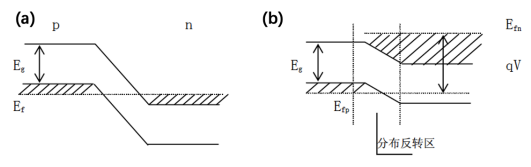
\includegraphics[width=1.0\linewidth]{img/1.png}
	\caption[半导体激光器能带示意图]{半导体激光器能带示意图}\vspace{1ex}
	\end{figure}
    \par 有些激光器是通过外加光源来提供能量实现粒子数反转, 有些激光器
    是通过外加电源注入载流子来实现粒子数反转, 半导体激光器属于后者.
    半导体中有若干光跃迁的方式, 而电子-空穴对辐射复合(激子复合)是其
    中主要的一种; 半导体激光器的发光原理就是, 在 p-n 节处产生粒子数反
    转, 使得大量电子和空穴复合, 从而实现了以半导体为增益介质的激光器.
    p-n 节的能带如上示意图所示: 在未加外电场的时候, p 区和 n 区费米能相
    等, 两区在接触的地方能带产生弯曲; p 区空穴更多, 因而费米面在价带
    以下; n 区电子较多, 因而费米面在导带以上. 而在 n 区被加了负电压,p
    区被加了正电压的时候(如上图右侧图所示; 即向 n 区注入电子, 向 p 区注
    入空穴), 导带电子数大大增多, 使得粒子数反转, 从而产生大量激子,
    形成增益介质.
    \par 激光器组成成分中还有谐振腔; 由于半导体的折射率比空气高很多,
    而且晶体的解理面很平整, 故半导体材料的解理面可以直接被用来构成激
    光器的谐振腔中的反射镜.
    	\begin{figure}[!h]
    	\centering
    	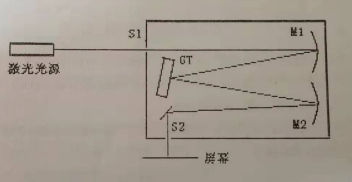
\includegraphics[width=.7\linewidth]{img/2.png}
    	\caption[单色仪的结构及光路]{单色仪的结构及光路}\vspace{1ex}
    	\end{figure}
\par 实验中先通过单色仪(图 2)测量半导体激光器的激光中心波长, 不过本次实验省略了这一步; 本实验中采用的半导体激光器波长为 550nm.
\begin{figure}[!h]
    	\centering
    	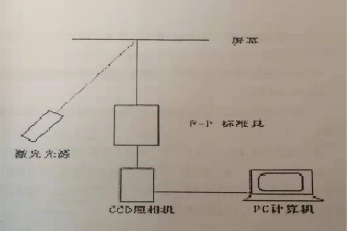
\includegraphics[width=.7\linewidth]{img/3.png}
    	\caption[测量谱线宽度光路图]{测量谱线宽度光路图}\vspace{1ex}
    	\end{figure}   
\par 第二步是测量半导体激光器谱线的宽度, 实验装置示意图如图 3 所示. 激光打到光屏上形成漫反射, 漫反射的光通过毛玻璃后进入 F-P 标准具形成等倾干涉, 毛玻璃的作用也是为了产生向各个方向传播的光; 在调节 F-P 标准具两个反射面平行之后, 利用得到的等倾干涉图样可以得到激光谱线宽度. 实验中并未使用 CCD, 而是直接利用手机拍摄的等倾干涉图样计算谱线宽度.具体来说:标准具产生干涉极大的条件为$2lcos\theta=k\lambda$, 光线经过焦距为 f 的透镜后成像在焦平面上, 利用小角近似及$\theta=D/2f$, D 为环的直径; 所以$2l(1-\dfrac{1}{8}(\dfrac{D}{f})^2)=k\lambda$; 同一干涉环的内径和外径分别为 $D_1$ 和 $D_2$,$k=2l/\lambda$, 则谱线宽度$\Delta\lambda=\dfrac{\lambda}{8f^2}(D_2^2-D_1^2)$. 而由于记录工具(手机摄像头)的焦距未知, 因而为了计算谱线宽度, 焦距要用其他量来代替. 实际上可以利用前后两个干涉环的数据来计算; 设两相邻
的干涉环外径分别为$D_a,D_b$,则$2l(1-\dfrac{1}{8}(\dfrac{D_a}{f})^2)=(k+1)\lambda,2l(1-\dfrac{1}{8}(\dfrac{D_b}{f})^2)=k\lambda$, 两式相减得$\dfrac{2l}{8f^2}(D_b^2-D_a^2)=\lambda$, 结合前面谱线宽度的表达式可得:$\Delta\lambda=\dfrac{\lambda^2}{2l}\dfrac{D_2^2-D_1^2}{D_b^2-D_a^2}$
\par 实验中由于半导体激光器强度过小使得看不到等倾干涉条纹, 因而换用 He-Ne 激光器(波长为 632.8nm)来进行实验.
\section{实验装置}
%	在此部分需要将实验条件交待清楚到别人能重复你的实验结果的程度. 此外,还需表明你已尽了最大努力来提高实验精度和结果的可靠性. 简单的不确定度估计可以在此节给出,复杂一些的可以放到分析讨论部分.\par
%	实验条件不仅是指直接影响实验结果的实验参量,而且还包括影响实验质量和可靠性的因素,如室温、空气湿度、基真空、原材料纯度等.\par
%	作为教学实验报告,此节写详细一点没有坏处.\par
%	成段有叙述,必要才分节。
%%%%%%%%%%%%%%%%%%%%%%%%%%%%%%

\section{结果与分析}
%	实验结果应尽量以图表的形式给出. 每一个图表都应该是完整的,即阅读图表时可以不必依赖正文.\par
%	依自己意愿,实验结果和对结果的分析讨论既可分为两节也可合在一节.\par
%	\begin{table}[h]
%	\caption{元件恒流大小,为什么要左对齐呢?奇怪。}
%	\small
%	\begin{tabularx}{.6\linewidth}{C{.3} C{1}}
%	\toprule
%	\midrule
%		元件\footnote{%
%			注释一个看看%
%		} & 恒流大小\footnote{%
%			再开一个!哈哈
%		} \\
%	\midrule
%		Pt  &
%			$\SI{1.00005}{\mA}
%				= \SI{100.005}{\mV} / \SI{100}{\ohm} $ \\
%	\midrule
%	\bottomrule
%	\end{tabularx}
%	\label{tab:ExTab}
%	\end{table}
%	
%	每个图一般包含:图名、轴名、轴、刻度、标尺、数据点、曲线、图例、标注和图注等部分. 应尽量让读者不看正文就能基本理解图的含意.\par
%	逐点测量得到的函数关系要同时用表格和图给出. 需要作比较的多条曲线要画在同一图上.\par
%	为避免读者在图表和正文间反复跳跃阅读,在正文中也要对图表作必要的说明.\par
%	
%	对于预料之外的实验结果,必须首先小心证明其可靠性.读者只有在相信你的实验结果时才愿意花时间看你的分析.\par
%	必须用文字归纳整理出正式的实验结果或结论.可信的实验结果是课程报告最重要的内容.作为一个实验物理工作者,分析解释出错并不丢脸,实验结果不被采信则是致命的.\par
%	教学实验的结论往往是预先知道的. 所以,教师更关心的是你的说理过程. 一般说来,单由课内实验的结果不足以能得到明确的结论. 此时,你可以引用他人的研究结果来帮助帮助自己的论证,但必须注明出处. \par
%	确实不能得到明确结论时,可以给出几种可能结论并指出可以再做哪些实验来帮助作进一步的判断.\par
%	总之,分析讨论部分要做到: 论据要valid,论证要reasonable,结论要convincing.\par
%%%%%%%%%%%%%%%%%%%%%%%%%%%%%%
\section{结论}
本实验中了解了利用 F-P 标准具测量激光谱线宽度的方法, 由于半导体激光器光强太弱没有测到相应结果; 测量了 He-Ne 激光器的谱线宽度, 为$(0.034\pm0.008)nm$; 并分析了误差来源. 本实验为以后进行相似的实验提供了经验.
\section{思考题}
1.能否正是在实验中测量的半导体激光器的线宽是真实线宽而不是 F-P 标准具的仪器线宽? 如何得到 F-P 标准具的线宽?
\par 答:需要测量 F-P 标准具的仪器线宽来确定测量得到的线宽是不是半导体激光器的真实线宽. 得到 F-P 标准具线宽的方法: 白光照明, 用滤光片使得大约只有 630-640nm 的光通过(范围不能太宽, 不然干涉调纹相互干扰; 不过用宽谱光照明然后将得到的干涉图样用 RGB 分解应该也可以,只是误差预计会比较大; He-Ne 激光器波长为 632.8nm), 利用同样的方法通过测量干涉环内外径得到相应谱线宽度; 如果 F-P 仪器线宽比测得的半导体激光器线宽小, 则测量到的线宽就是半导体激光器的真实线宽, 反之则与真实线宽之间有误差.

2.要测量谱线宽度为 0.01 埃的谱线, 本实验装置要做哪些改变? 
\par 答:F-P 标准具的能分辨的最小波长差可能大于 0.01 埃, 因而需要将其换成分辨率更高的光谱仪, 或提升其性能.

3.温度变化对谱线宽度有什么影响? 设想一个观察温度效应的实验方案. 
\par 答:半导体激光器中有声子的热效应, 使得产生辐射的电子空穴对的能量有一定涨落, 因而温度低的时候谱线宽度会更窄. 同时声子的效应可能也
会产生一些其他的谱线.\\
实验方案: 将半导体激光器放在密闭盒子里(盒子里面盛有液氮), 利用液氮对其降温, 测量不同温度时的激光波长和谱线宽度.

4.根据光谱线宽度的定义分析实验测量结果的误差. 提出一种精确测量谱线宽度的方案. 
\par 答:\\1.如果 F-P 标准具两个平面没有调平行, 则不同位置的光产生干涉极大的条件不同, 会使得总体的干涉情况不如完全平行时理想,会使得 F-P 标准具分辨本领下降.实验中假设这一部分没有误差.2.前面推导中所用小角近似也会产生误差.3.对干涉条纹内外径判断有偏差会产生误差.\\
因为F-P仪的色分辨能力与反射率R正相关,所以采用 R 更大的材料或者采用级次更高的腔(即增大腔长)能使得分辨率更高.或者换用光栅分光,接透镜成像,扫描像面不同位置光强得到相应的光谱. 
\section{致谢}
%	此部分感谢同组人...和对实验和报告有帮助的人.
	感谢我的合作伙伴杨轩同学,他的工作是不可或缺的;感谢耐心的胡小永指导老师对我们的巨大帮助。
\begin{thebibliography}{99}
	\addcontentsline{toc}{section}{参考文献}
	\bibitem{ref1}北京大学物理学院光学所, 激光实验, 第二版, 北京: 北京大学物理学院, 2023.
\end{thebibliography}
\clearpage
\end{document}
